\section{Проектування мультиагентної системи}
\subsection{Розробка вимог до програмної системи}
\subsubsection{Галузь застосування}
Даний програмний продукт може бути використаний логістичними компаніями з метою покращення сервісу, викладачами та студентами для дослідження логістичних систем.

\subsubsection{Бізнес вимоги}
Необхідно розробити програмний компонент для моделювання розподільчих логістичних систем різних конфігурацій з метою оцінки кожної з конфігурацій.

\subsubsection{Функціональні вимоги}
Специфікацію функціональних вимог у вигляді \acrshort{uml}-діаграми прецедентів представлено на рисунку~\ref{fig:system_usecase}.

\begin{figure}[H]
	\centering

	\tikzumlset{font=\footnotesize} 
	\tikzumlset{fill usecase=white}
	\begin{tikzpicture} 
		\umlactor[x=4, y=2]{Актор} 
		\umlusecase[x=1, y=0, width=3.5cm, name=service]{Перегляд параметрів системи у реальному часі} 
		\umlusecase[x=0, y=3, width=3.5cm, name=export]{Експорт конфігурації до \acrshort{json} файлу}

		\umlusecase[x=7, y=1, name=report]{Генерація звіту} 
		
		\umlusecase[x=11, y=5, name=report_c_period]{Вибір типу даних} 
		\umlusecase[x=9, y=3, name=report_c]{Конфігурація звіту} 
		\umlusecase[x=11, y=1, name=report_c_actors]{Вибір акторів}  

		\umlassoc{Актор}{service}
		\umlassoc{Актор}{export}
		\umlassoc{Актор}{report}

		\umlinclude{report}{report_c}
		\umlextend{report_c_period}{report_c}
		\umlextend{report_c_actors}{report_c}
	\end{tikzpicture}

	\caption{\acrshort{uml}-діаграма прецедентів системи}
	\label{fig:system_usecase}
\end{figure}

Список функціональних вимог системи:
\begin{enumerate}[label={\arabic*)}]
	\item система повинна мати можливість імпорту початкової конфігурації логістичної системи з \acrshort{json} файлу;
	\item система повинна автоматично приймати рішення о розподілі матеріальних потоків;
	\item система повинна мати графічний інтерфейс перегляду поточного стану логістичної системи: рівень запасу товарів, рівні сервісу, рівень ризику, навантаження мережі. 
	\item система повинна мати можливість генерації звіту.
\end{enumerate}

Генеруємий звіт та графічний інтерфейс програмної системи повинен включати (для кожній ітерації та агенту системи) рівень логістичного сервісу, перенапружені ланки логістичної системи, прогнозуємий рівень збиту, показники ризику.

\subsubsection{Нефункціональні вимоги}
Список нефункціональних вимог системи:
\begin{enumerate}[label={\arabic*)}]
	\item система повинна бути платформонезалежною та підтримувати такі операційні системи, як Debian, Windows, macOS;
	\item система повинна мати зручний інтерфейс;
	\item система повинна мати високий рівень масштабованості;
	\item система повинна мати теоретичну можливість додавання нових агентів зі своєю поведінкою.
\end{enumerate}

\subsection{Архітектура програмної системи}
Для реалізації системи була обрана однорівнева архітектура \textit{(standalone application)}.

Однорівнева архітектура була обрана через те, що користувач буде проводити дослідження з використанням розробленої системи на машині з налаштованою системою. 
На даний момент немає сенсу розробляти багаторівневу архітектуру системи, бо продукт не є масовим.

\subsubsection{Діаграма компонентів}
На рисунку~\ref{fig:system_component} зображена діаграма компонентів системи.

\begin{figure}[H]
	\centering
	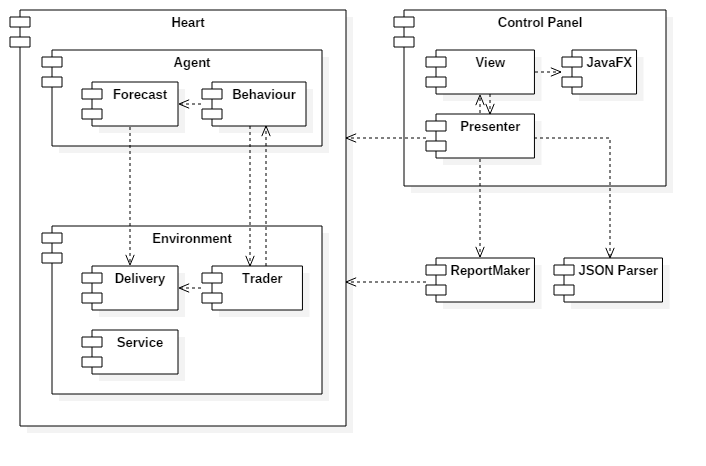
\includegraphics[width=\textwidth]{system_components}
	\caption{\acrshort{uml}-діаграма компонентів системи}
	\label{fig:system_component}
\end{figure} 

Головними компонентами є:
\begin{itemize}
	\item \texttt{Heart} --- платформа для асинхронного запуску та взаємодії агентів;
	\item \texttt{Agent} --- актори розподільчої логістичної системи;
	\item \texttt{Environment} --- навколишня середа агентів;
	\item \texttt{Control Panel} --- графічний інтерфейс користувача;
	\item \texttt{ReportMaker} --- створення звіту;
	\item \texttt{JSON Parser} --- запис та читання з \acrshort{json}-формату;
	\item \texttt{Presenter} --- взаємодія інтерфейсу з агентною платформою.
\end{itemize}

\subsubsection{Діаграма класів}
На рисунку~\ref{fig:system_class} зображена діаграма класів системи.

\begin{figure}[H]
	\centering
	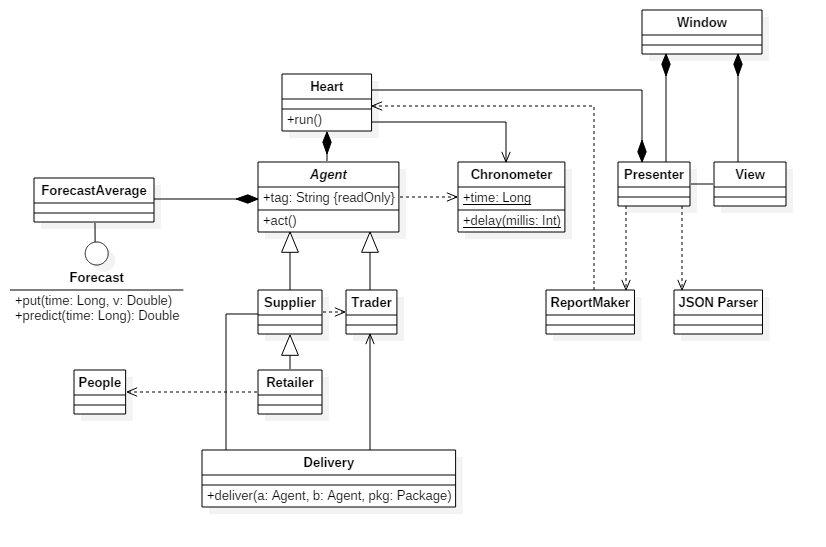
\includegraphics[width=\textwidth]{system_class}
	\caption{\acrshort{uml}-діаграма класів системи}
	\label{fig:system_class}
\end{figure} 

Головними класами є:
\begin{itemize}
	\item \texttt{Heart} --- керує асинхронним запуском та взаємодією агентів;
	\item \texttt{Agent} --- базовий клас який не має поведінки;
	\item \texttt{Supplier} --- агент-постачальник;
	\item \texttt{Retailer} --- агент-роздрібний-продавець;
	\item \texttt{Delivery} --- сервіс доставки замовлень;
	\item \texttt{Trader} --- агент-трейдер, який керує активними тендерами;
	\item \texttt{Observer} --- слідкує за поточним станом агентів та надає інформацію про них;
	\item \texttt{Chronometer} --- операції з поточним часом системи;
	\item \texttt{ForecastAverage} --- прогнозування методом ковзної середньої.
\end{itemize}

\subsubsection{Діаграма послідовності}
На рисунку~\ref{fig:system_sequence} зображена спрощена діаграма послідовності системи.

\begin{figure}[H]
	\centering
	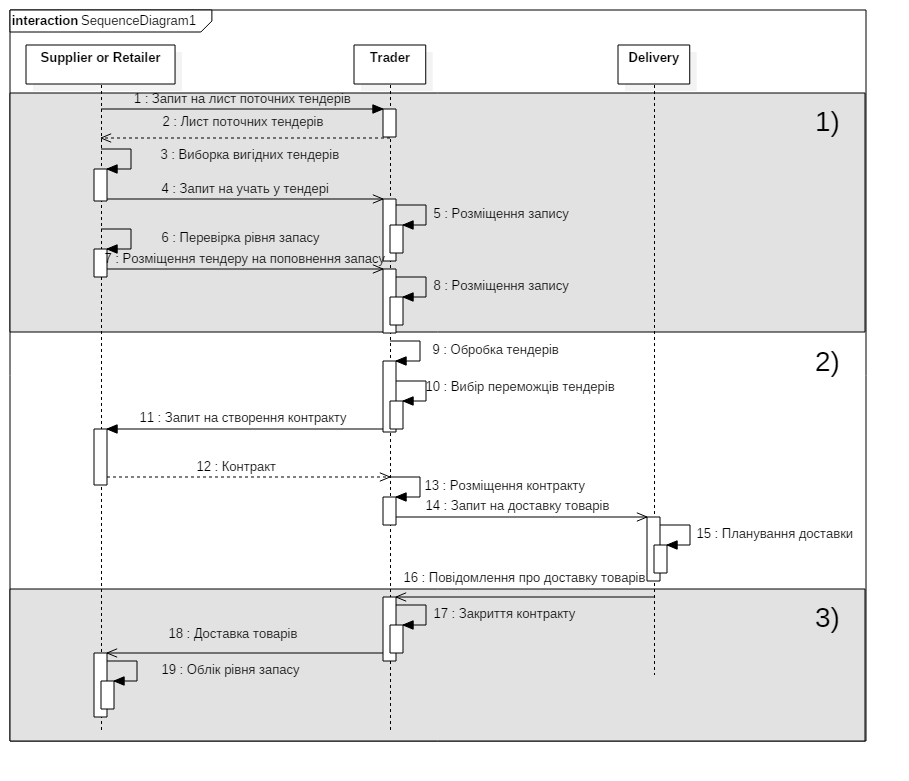
\includegraphics[width=\textwidth]{system_sequence}
	\caption{\acrshort{uml}-діаграма послідовності}
	\label{fig:system_sequence}
\end{figure} 

На діаграмі позначено:
\begin{enumerate}[label={\arabic*)}]
	\item спрощений життєвий цикл постачальника та роздрібного торговця;
	\item спрощений життєвий цикл трейдера;
	\item спрощений життєвий цикл системи доставки.
\end{enumerate}

\subsubsection{Діаграми активності}
На рисунку~\ref{fig:system_retailer_activity} зображена діаграма активності життєвого циклу роздрібного продавця.

\begin{figure}[H]
	\centering
	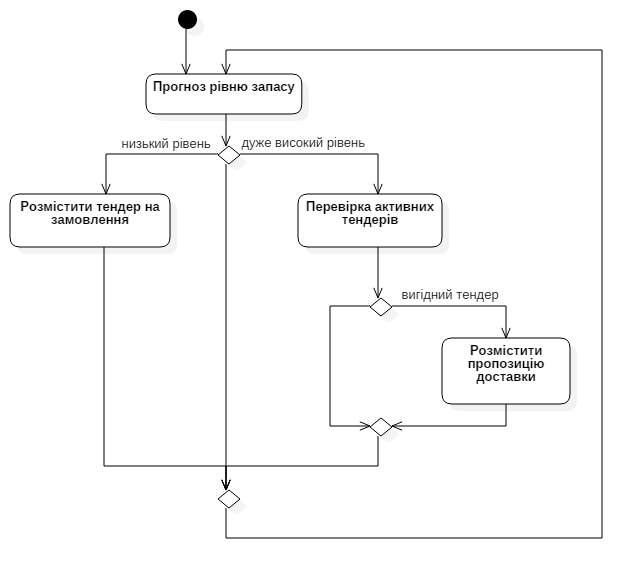
\includegraphics[width=0.75\textwidth]{system_retailer_activity}
	\caption{\acrshort{uml}-діаграма активності життєвого циклу роздрібного продавця}
	\label{fig:system_retailer_activity}
\end{figure} 

\subsection{Обґрунтування вибору платформи розробки та інструментальних засобів}
\subsubsection{Мова програмування Kotlin}
Основна мета мови Kotlin --- запропонувати більш компактну, продуктивну і безпечну альтернативу мови Java, придатну для використання всюди, де сьогодні використовується Java.
Kotlin чудово підходить для розробки серверних застосунків, дозволяя писати стислий та експресивний код.
Переваги Kotlin~\cite{kotlin,Panchal2017}:  
\begin{enumerate}[label={\arabic*)}]
	\item експресивність --- інноваційні можливості Kotlin, такі як типо-безпечні конструктори та делегати, дозволяють створювати потужні та прості у використанні абстракції;
	\item масштабованість --- підтримка Kotlin корутин \textit{(coroutines)} допомагає створювати масштабовані застосунки;
	\item сумістність --- Kotlin повністю сумісний зі всіма Java фреймворками;
	\item міграція --- Kotlin підтримує покроковий перехід з кодової бази на Java;
	\item інструменти --- Kotlin добре підтримується середовищами програмування;
	\item легкість навчання --- для Java розробника дуже легко почати вивчати Kotlin.
\end{enumerate}

\subsubsection{Система управління версіями Git}
Використання системи контролю версії є необхідним для роботи над великими проектами.

Система контролю дозволяє зберігати попередні версії файлів та завантажувати їх за потребою. 
Вона зберігає повну інформацію про версію кожного з файлів, а також повну структуру проекту на всіх стадіях розробки.

Git --- розподілена система керування версіями файлів та спільної роботи. Git є однією з найефективніших, надійних і високопродуктивних систем керування версіями, що надає гнучкі засоби нелінійної розробки, що базуються на відгалуженні і злитті гілок~\cite{Chacon2009}.

\subsubsection{Середовище розробки застосунків Intellij IDEA}
IntelliJ IDEA --- інтегроване середовище розробки програмного забезпечення багатьма мовами програмування. 
Community версія середовища IntelliJ IDEA підтримує інструменти для проведення тестування TestNG і JUnit, системи контролю версій CVS, Subversion, Mercurial і Git, засоби збирання Maven і Ant, мови програмування Kotlin, Java, Java ME, Scala, Clojure і Groovy. 
Середовище містить редактор регулярних виразів, систему перевірки коректності коду, система контролю за виконанням завдань та ін.~\cite{Kalinichenko2013}.

Середовище IntelliJ IDEA є рекомендованим для розробки застосунків на мові програмування Kotlin~\cite{kotlin}.

\subsubsection{Аналіз та вибір агентної платформи}
Агентна платформа --- це проміжний виконавчий рівень, який знаходиться між агентами та операційною системою.
Існує велика кількість різноманітних агентних платформ, які значно спрощують розробку \acrshort{mas}~\cite{Kravari2015}.
При реалізації \acrshort{mas} можна виділити три основних підходи до розробки~\cite{Zhou2010}:
\begin{enumerate}[label={\arabic*)}]
	\item програмування агентної системи за допомогою \acrshort{fipa} фреймворків;
	\item програмування агентної системи без використання фреймворків;
	\item використання графічних пакетів розробки для побудови \acrshort{mas}.
\end{enumerate}

У таблиці~\ref{tab:mas_platform_comparsion} приведено порівняння цих платформ.

Для розробки було прийнято рішення писати свою легку платформу для запуску агентів через те, що готові фреймворки для побудови агентних систем мають надмірний функціонал та складні у використанні і вивченні.
